\begin{IEEEbiography}[{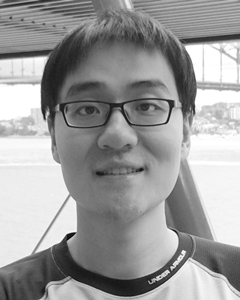
\includegraphics[width=1in,height=1.25in,clip,keepaspectratio]{figures/fan.png}}]{Taosha Fan}
received his B.E. degree in automotive engineering from Tongji University, Shanghai, China, in 2013, and M.S. degrees in mechanical engineering and mathematics from Johns Hopkins University, Baltimore, MD, USA, in 2015. He is currently a Ph.D. candidate in mechanical engineering at Northwestern University, Evanston, IL, USA. His research interests lie at the intersection of robotic control, simulation and estimation.
\end{IEEEbiography}

\begin{IEEEbiography}[{
\includegraphics[width=1in,height=1.25in,clip,keepaspectratio]{figures/murphey.png}}]{Todd Murphey}
received his B.S. degree in mathematics from the University of Arizona and the Ph.D. degree in Control and Dynamical Systems from the California Institute of Technology.
He is a Professor of Mechanical Engineering at Northwestern University. His laboratory is part of the Neuroscience and Robotics Laboratory, and his research interests include robotics, control, computational methods for biomechanical systems, and computational neuroscience.
Honors include the National Science Foundation CAREER award in 2006, membership in the 2014-2015 DARPA/IDA Defense Science Study Group, and Northwestern’s Professorship of Teaching
Excellence. He was a Senior Editor of the IEEE Transactions on Robotics.
\end{IEEEbiography}